\documentclass[a4paper]{scrartcl}

% Localization
\usepackage[english]{babel}
\usepackage[T1]{fontenc}
\usepackage[utf8]{inputenc}

% Quotations
\usepackage{dirtytalk}

% PDF-compatible landscape mode
\usepackage{pdflscape}

% Advanced tables
\usepackage{array}
\usepackage{tabularx}

% Fancy tablerules
\usepackage{booktabs}

% Graphics
\usepackage{caption}
\usepackage{subcaption}
\usepackage{graphicx}
\graphicspath{{resources}}

% Decent quotations
\usepackage{csquotes}

% Automatic float barriers to each \section
% \usepackage[section]{placeins}

% Math
\usepackage{amssymb,amsmath,amsfonts}
\usepackage{mathtools}

% Algorithms
\usepackage{algpseudocode}

% SI units
\usepackage[binary-units]{siunitx}

% Clickable links in PDF
\usepackage{hyperref}

\title{11043 - Internet of Things - Summary} % Title
\author{Michael Senn}
\date{\today}

\begin{document}

\maketitle % Inserts the title, author and date

\tableofcontents

\section{Introduction}

\subsection{Sensor networks}

\begin{description}
		\item[Sensor network] Deployment of small, inexpensive self-powered
				devices which can sense, communicate and compute. Size-limited
				by battery.
		\item[Sink] Gateway between fixed and wireless sensor network. Controls
				and manages sensor nodes.
		\item[Challenges] Finite energy \& computation resources, network
				capabilities, unreliable hardware and network, need for
				synchronization (time, location)
		\item[Data dissemination] Observer-initiated (on-demand), event-driven
				(by sensor nodes), continuous (pre-specified rate)
		\item[Transmission and reception costs] Much higher than computations
\end{description}

\subsection{Advanced WSN structures}

\begin{description}
		\item[Mobile WSN] Static: Need dense deployment. Fully mobile
				(sensors are moving): Weight constraints, communication
				challenging. Hybrid (fixed base stations, mobile sensors
				carried by humans/vehicles/...)
		\item[Participatory sensing] Using sensors of end-user devices as part
				of network
		\item[WSAN]: Includes actuators, acting on sensor data
		\item[M2M communications]
		\item[IoT] Physical things having counterpart in network, exposing
				data, acting on commands.
		\item[CPS] Control/computing co-design, actor/sensor networks
		\item[Multimedia WSN] Inclusion of multimedia traffic, e.g.
				surveillance. Requirements for encoding, bandwith, QoS
\end{description}

\subsection{WSN Applications}

WSN applications can be classified by goal, connectivity, mobilitiy, data
rates, ...

\begin{description}
		\item[Querying] Sensors collect data, applications queries data from
				sensors. Potentially aggregation/filtering within WSN.
		\item[Tasking] Sensors programmed to perform actions on events, e.g.
				send message when reading exceeds threshold. Combined with
				actuators (e.g. building control)
\end{description}


\section{Hardware platforms}

\subsection{RFID - Radio frequency identification}

\begin{itemize}
		\item Passive tags get energy from received signal
		\item Active tags on-board battery
		\item Near-field communication: Data and power transmission via
				magnetic field to tag. Tag's data affects magnetic field, which
				is measured by RFID reader.
		\item Far-field communication: EM used to transfer power to tag, EM
				backscatter to send data from tag to RFID reader. Up to
				\SI{100}{\meter}
		\item NFC is a form of RFID at \SI{13.56}{\mega\Hz}, with two-way communication
\end{itemize}

\subsection{Sensor nodes}

\begin{description}
		\item[Energy-efficiency] Tradeoff: General-purpose hardware less efficient than embedded
				processors. ASICS inbetween.
		\item[Tiered network architecture] Sensor nodes with low computing
				resources, report to computing nodes which aggregate. Those to
				delivery nodes with high bandwith, which send to gateway nodes
				which are hooked up to the internet. Allows most nodes to be
				cheap, expensive operations to take place at nodes with static
				power supply.
		\item[Multi-processor nodse] Multiple simpler processors, flexibile
				energy saving by only turning on what's needed.
\end{description}

Classification of sensor node hardware:
\begin{description}
		\item[System-on-Chip]: RF (radio), CMOS (transistors), MEMS (mechanical
				system) on single chip. Low power, small nodes. Special
				instruction sets, limited support for reprogramming. Example: PicoNode.
		\item[Dedicated embedded nodes] Commerical OTS chip sets, low-power
				processing and communications. Full hardware access, C or ASM.
				Example: TelosB.
		\item[General-purpose computers] Based on PCs or PDAs, OTS OS and
				applications. Standard communication (bluetooth, wireless,
				...). High flexibility. Example: Raspberry Pi.
\end{description}


\subsection{Energy sources}

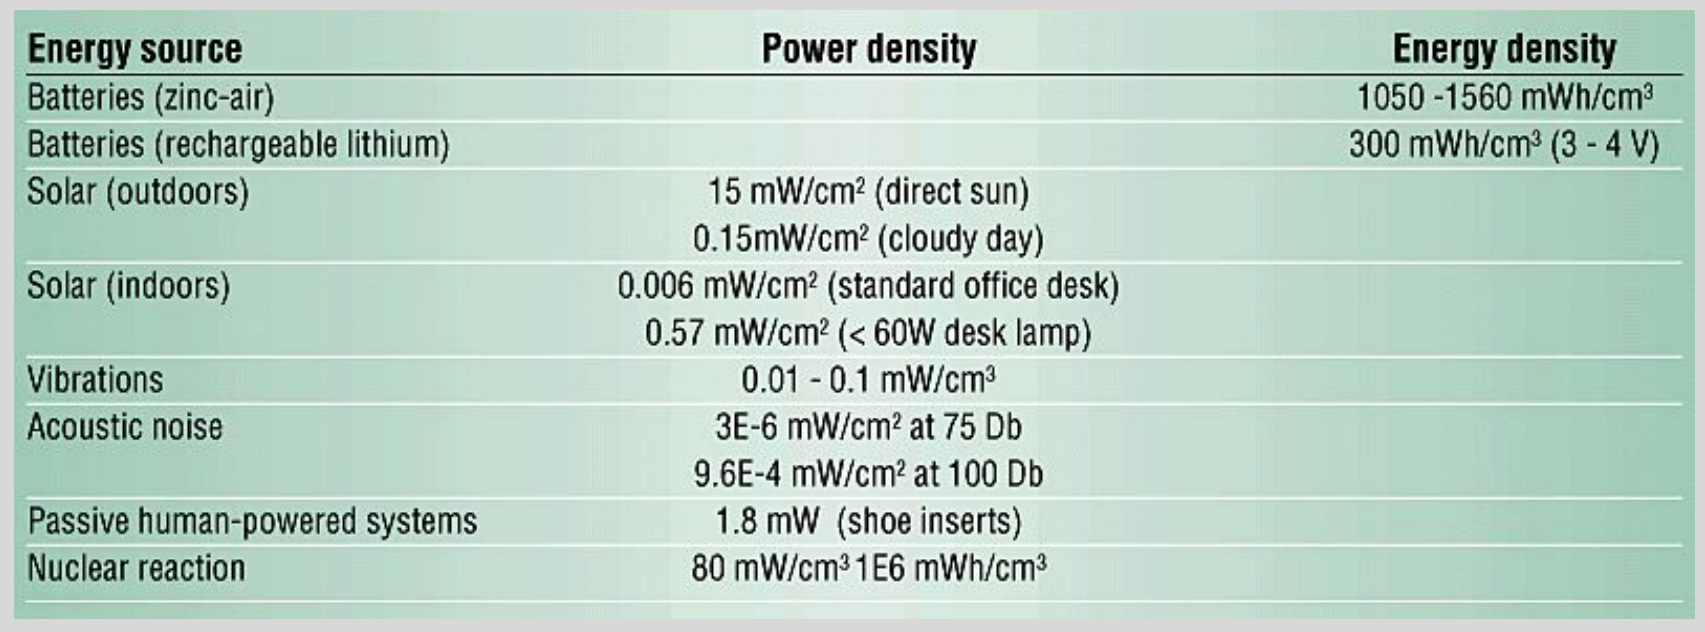
\includegraphics[width=\textwidth]{02_energy_sources}

\begin{description}
		\item[Energy scavenging] Photovolatic, temperature gradients, vibratinos, ...
\end{description}

\subsection{Energy saving in sleep mode}

Given power consumption active / sleep $P_{active}$ and $P_{sleep}$, $t_1$ time
when sleep mode entered, $t_{down}$ when fully powered down, $t_{event}$ when
waking up, then $E_{saved}$ energy saved, $E_{overhead}$ overhead due to sleep.
Sleep mode beneficial if $E_{saved} > E_{overhead}$. Where:

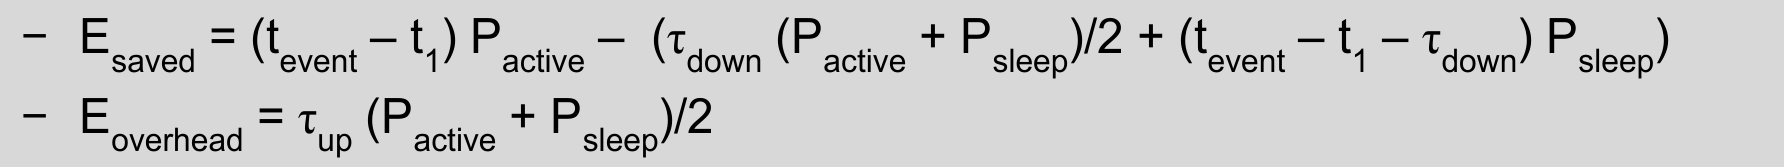
\includegraphics[width=\textwidth]{02_energy_saving}

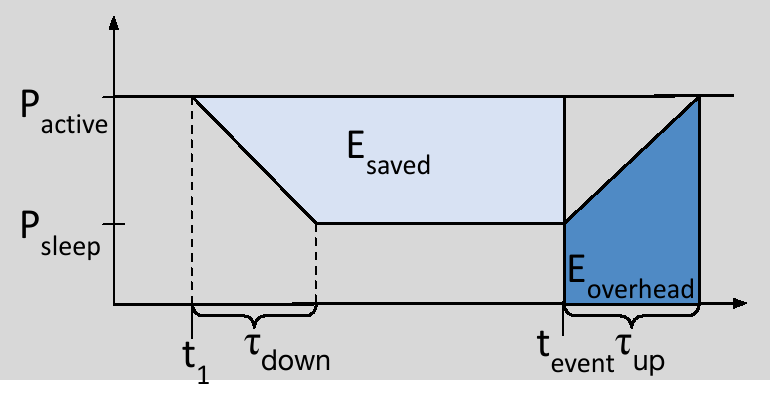
\includegraphics[width=0.5\textwidth]{02_energy_saving_model}

\subsection{Dynamic Voltage Scaling}

Switching power dissipated (= losses!) by capacitor is $P_{dynamic} = C \cdot F
\cdot V^2$, $C$ capacity, $F$ switching frequency, $V$ supply voltage. Dynamic
voltage scaling allows reducing power consumption in embedded system, by
reducing switching losses, by reducing voltage and frequency of processors.

\subsection{Transceiver}

\begin{itemize}
		\item Offers service (packet, byte, bit) to upper layer
		\item States: Transmit, receive, idle, sleep
		\item Handles modulation, coding, carrier-sensing, ...
		\item Often large startup time and cost when starting to send
		\item Ideally transmit few large packets instead of many small
\end{itemize}

\subsection{Multi-hop communication}

Energy cost over $d$ distance roughly $E \approx d^n$, where $n$ is path loss
factor of $2$ to $4$. Multi-hop communication can be way cheaper:

\begin{align*}
		E(h, d) = h \cdot(\alpha + \beta \cdot \frac{d}{h}^n)
\end{align*}

Where $\alpha$ sum of distant-independent components (eg receiver, startup,
...), $\beta$ distant-dependant terms eg power amplifier, path loss.


\section{Operating systems}

\begin{description}
		\item[Node-centric operating systems] Simplified versions of normal
				operating systems, providing abstraction of node to
				programmers. Example: MANTIS, RIOT.
		\item[Node-level progrmaming tools] Platform providing components to
				programmer. Example: TinyOS, Contiki.
\end{description}

\subsection{Concurrency}

\begin{description}
		\item[True vs pseudo] Multi-process (requries multiple processors) vs
				sequential
		\item[Event-driven] Kernel invokes event handlers when
				event occurs. One event runs at a time. Event
				handler runs to completion.
				\begin{itemize}
						\item Cheap pseudo-concurrency, complements networking protocols, inexpensive
						\item Program must be chopped into subprograms, high learning curve
				\end{itemize}
		\item[Multi-threading] Threads are waiting for events.
				Kernel unblocks threads when event occurs.
				Threads run until next blocking statement. Each
				thread requires stack, but long operations
				possible.
				\begin{itemize}
						\item Programmer in control. Real-time performance.
								Better simulation of true concurrency.
						\item High memory footprint. Complex shared memory.
								Expensive context switches.
				\end{itemize}
		\item[Mix: Threads on top of event-driven kernel] Kernel is
				event-based, multi-threading as library, used by tasks where
				required.
\end{description}

\subsection{TinyOS}

\begin{itemize}
		\item Simplifications: No FS, static memory allocation, thread support by application level library, minimal network abstractions
		\item Each application built into the operating system
		\item Concurrency left to programmer, event model
		\item Applications written in nesC, static language (no dynamic memory allocations!), support for even-tbased TinyOS design
		\item Events: Interrupts by clock, radio, ..., execute event handlers which run to completion
		\item Tasks: Created by component, posted to task scheduler. Run to completion, a form of deferred computation.
		\item Separation of method call initiation and return of call, compare async methods
		\item Commands flow to lower components, events back to higher ones
\end{itemize}

\subsection{ContikiOS}

\begin{itemize}
		\item Event-driven kernel with preemptive multitasking
		\item Core OS as binary image, programs loaded by loader
		\item Kernel dispatches events to processes, which define event handlers and optional polling handlers to poll hardware state
		\item Process state stored in its own memory. Processes share address space, no memory protection.
		\item Event scheduler handles async and sync events. Async are
				dispatched at some point, synchronous execute event handler
				immediately, then return.
		\item Event handlers run to completion
		\item $\mu$-IP, small TCP/IP stack with support for IPv4/6. Largely RFC-compliant.
\end{itemize}

\subsubsection{Protothreads}

\begin{itemize}
		\item Stackless
		\item Local variables not preserved across blocking statements
		\item But no need to run to completion, as only have to run to next blocking statement
\end{itemize}

\subsection{MANTIS OS}

\begin{itemize}
		\item Layered multi-threaded OS. Nearly a full OS.
		\item Global variables allocated at compile time, rest managed as heap. Stack for each thread frmo heap.
		\item Fixed size thread table.
		\item HW interrupts sent to drivers. No SW interrupts. Timer interrupts handled by kernel.
		\item Different options for network stack.
		\item Power management via sleep. When all threads asleep, OS shuts down microcontroller.
		\item Dynamic reprogramming possible. (eg OTA)
\end{itemize}

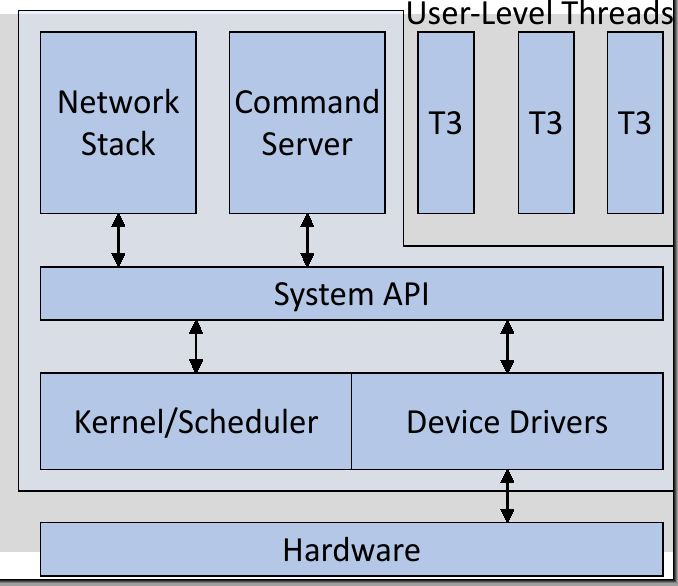
\includegraphics[width=0.5\textwidth]{03_mantis}

\subsection{RIOT}

\begin{itemize}
		\item Microkernel with multithreading
		\item Static memory allocation
		\item TCP/IP stack
		\item Scheduler switches to idle (sleep) thread when nothing to do,
				wakes up on interrupts (external or kernel-generated)
\end{itemize}

\subsection{OS power management}

\subsubsection{Low-Energy Earlierst Deadline First Scheduling (LEDF)}

CPU-centric.

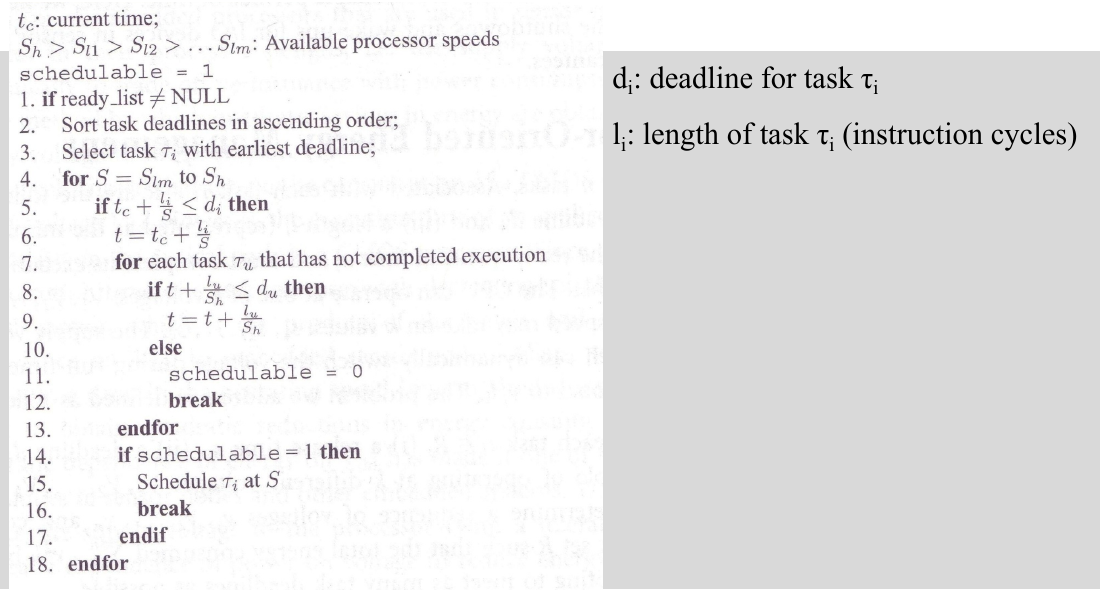
\includegraphics[width=\textwidth]{03_ledf}

\subsubsection{Low-Energy Device Scheduling (LEDES)}

I/O-centric.

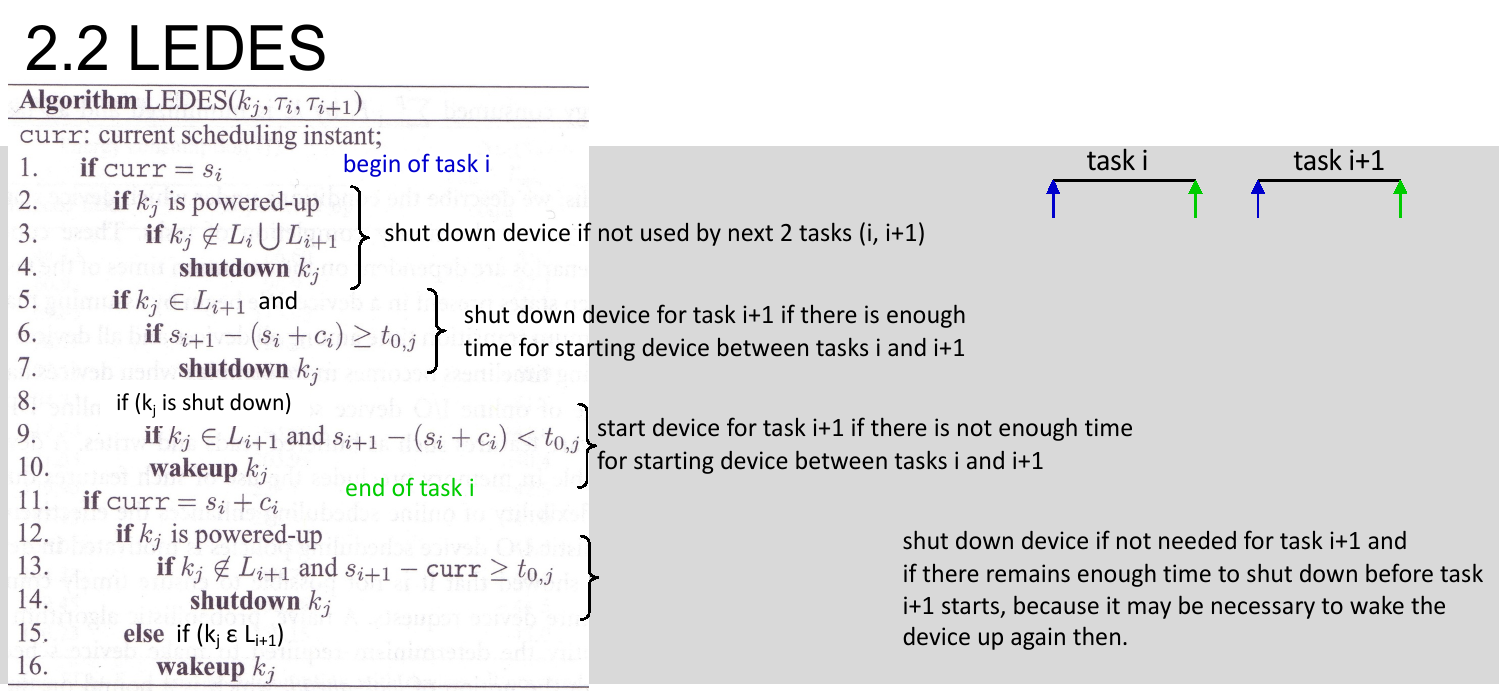
\includegraphics[width=\textwidth]{03_ledes}


\section{Localization}

Localization mechanisms:

\begin{description}
		\item[Coordinate systems] Absolute (global), relative (to local point, known by full network), local (to commmunicating parties)
		\item[Algorithms] Centralized, distributed, localized
		\item[Measurement parameters] Distances (lateration), angles (angulation)
		\item[Range-free vs range-based] Range-measurements, using eg received
				signal strength for distance estimation. Range-free, using
				connectivity information (lower accuracy, lower hardware
				requirements)
\end{description}


\subsection{Distance estimation}

\subsubsection{Time of arrival}

Distance $d = ((T_3 - T_0) - (T_2 - T_1)) \cdot v / 2$.
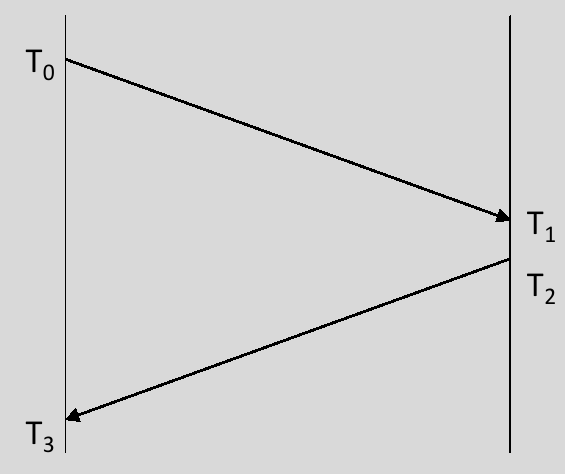
\includegraphics[width=0.5\textwidth]{04_time_of_arrival}

Example: Time-of-flight sensor network ranging.

\subsubsection{Time difference of arrival}

Transmission of two different signals from a single point. Either to same
source (two signal types, eg ultrasound and radio waves), or to two landmarks.
Signal transmission time irrelevant. Each measurement defines a hyperbola,
intersection of two provides a fixed distance (but not position!).

Distance $d = ((T_3 - T_1) - (T_2 - T_0)) \cdot (v_1 \cdot v_2) / (v_1 - v_2)$.

Example: Cricket.

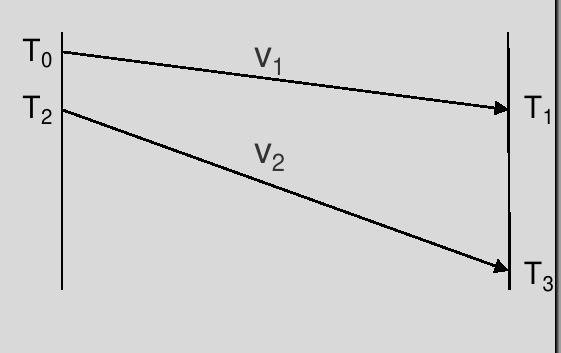
\includegraphics[width=0.5\textwidth]{04_time_difference_of_arrival}

\subsubsection{RSSI}

$PL$ path loss, $d_0$ nearby reference point, $n$ loss coefficient. Then $PL(d)
= PL(d_0) + 10 \cdot n \cdot \log(\frac{d}{d_0})$.

Problem: Unstable path loss / distance curve due to environmental conditions.

\subsubsection{Lighthouse location system}

Assumption: Parallel beam of width $b$ transmitted from lighthouse. Each node
measures time $t_{beam}$ it saw the beam. $t_{turn}$ time for beam to do one
rotation. Then:

\begin{align*}
		d = \frac{b}{2 \cdot \sin(\pi \cdot \frac{t_{beam}}{t_{turn}})}
\end{align*}

Problem: Parallell beam might be hard to realize, but can be improved with two
lighthouses.

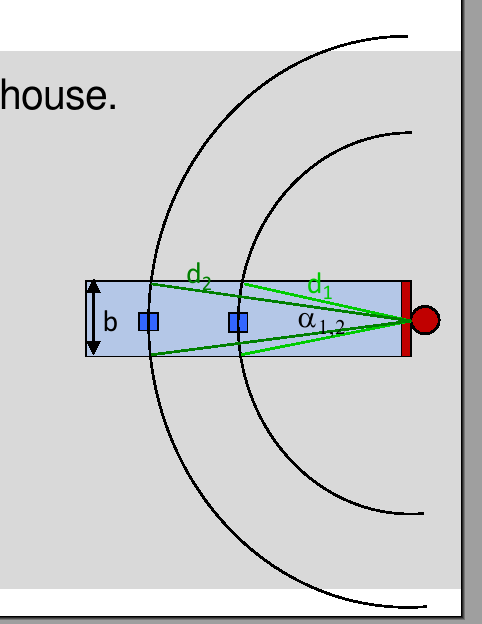
\includegraphics[width=0.5\textwidth]{04_lighthouse}

\subsection{Angle estimation}

Can be done using directional antennas, or phase/time difference of signal
arrival from multiple antennas.

\subsubsection{Beam forming}

Directional antenna allows detecting direction of signal, and hence angle to
signal source.

\subsubsection{VHS omni-directional ranging}

Landmark sends two signals: One periodic and omni-directional with period $p$,
one directional and rotating. Node measures time difference $d$ between first
and second signal, then $\alpha = d / p \cdot 2 \pi$.

\subsubsection{RSS estimation}

Ratio of RSS between two directional antennas depends on angle of signal.

\subsubsection{Compass}

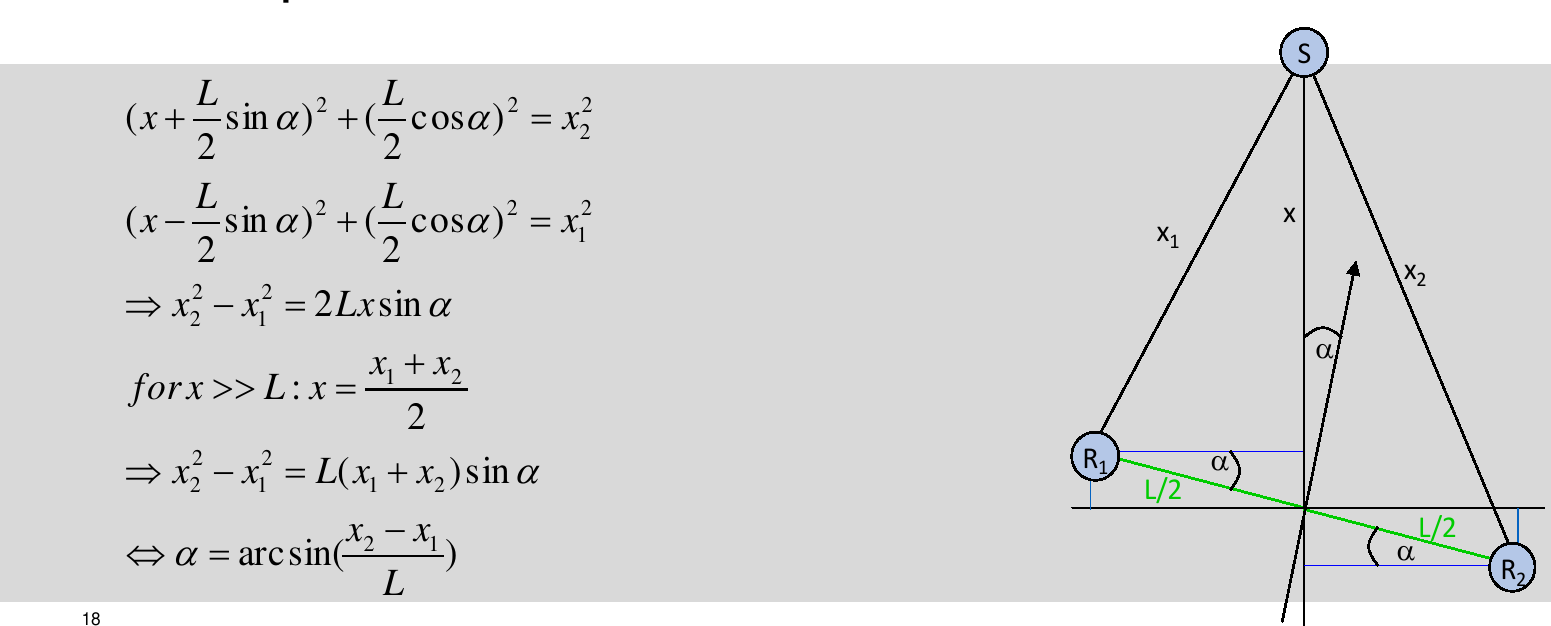
\includegraphics[width=0.8\textwidth]{04_compass}

\subsection{Range-based localization}

\subsubsection{Bounding box}

Boxes around anchor nodes where distance is known. Intersection of boxes is
bounding box for location.

\subsubsection{Weighted centroid}

Set of anchor nodes with known positions $x_i$. Weights $\omega_i$ dependant on
eg number of beacons from node, RSSI, etc. Then position:
\begin{align*}
		x = \frac{\sum_{i = 1}^N \omega_i \cdot x_i}{\sum_{i = 1}^N \omega_i}
\end{align*}

\subsubsection{Trilateration \& multilateration}

Distance measuremetns to landmark nodes. Curves have intersections, 3
measurements for position in plane (assuming everyone on ground!). Errors can
cause an area instead of a single point, redundant measurements with
least-squares compensation can help.

Multilateration extends by using >3 landmark nodes. Given distances $d_i$ to
nodes with positions $(x_i, y_i$), linearization of the $(x_i - x)^2 + (y_i -
y)^2 = d_i^2$. Then solving overdetermined system with e.g. least-squares.

\subsubsection{Triangulation}

Nodes measure angles to landmarks. Circles denote points with same angle to two
points, node must then lie oncircle intersections.

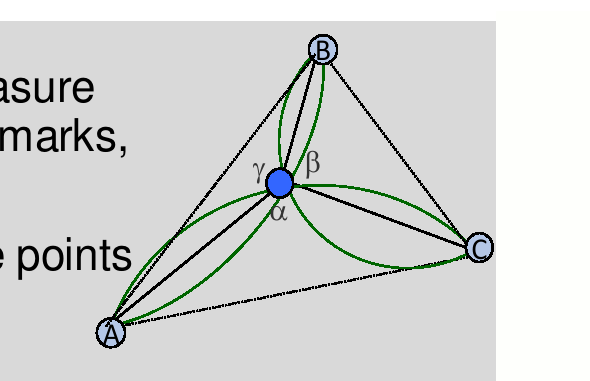
\includegraphics[width=0.5\textwidth]{04_triangulation}

\subsubsection{Fingerprinting}

Comparison of received signal patterns with database. Requires offline
collection phase where signals from base stations at various positions
measured. Then on-line phase where e.g. nearest-neighbour-signal-space
minimizes distance to known DB entries. Optionally use average of closest $k =
2, 3, 4$ DB entries as position.

\subsection{Range-free localization}

Techniques based on information of network area (eg overlapping transmission
ranges), hop count, neighbours, ...

\subsubsection{Approximate point in triangle}

Node detects whether inside or outside of triangles of its neighbours. Node
must then be in intersection of triangles it is within.

If node able to move: Perfect triangulation test possible by moving node. If
inside triangle, moving any direction will bring you closer to at least one
corner, and farther from at least one corner. If outside triangle, there must
exist a direction where it gets closer to, or farther from, all corners.

Otherwise, approximate point-in-triangulation test by estimating distance from
neighbours using eg RSSI. If any of its neighbours is closer/farther than
itself from all corners, its neighbour (and by assumption the node itself) must
be outside. Otherwise, its neighbour (and the node itself) inside the triangle.

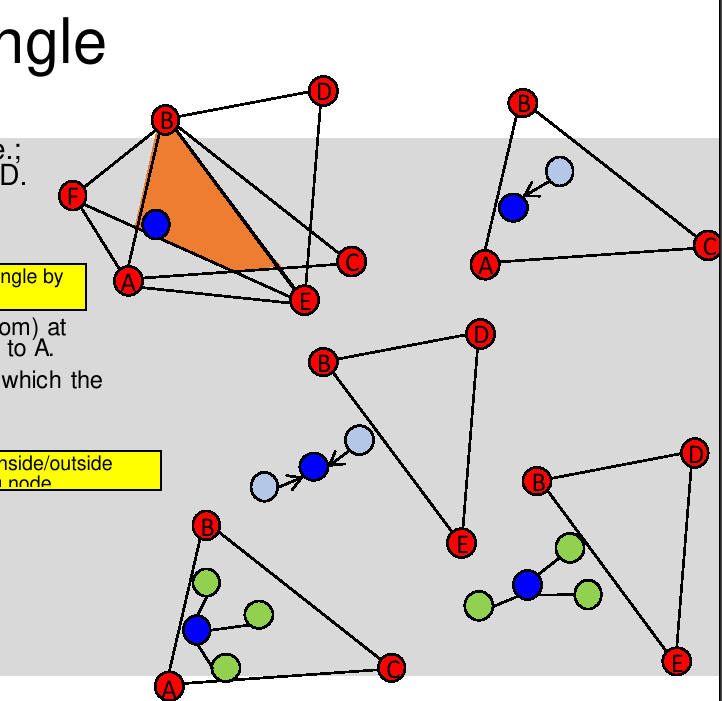
\includegraphics[width=0.6\textwidth]{04_approximate_point_in_triangle}

\subsection{Localization in multi-hop environments}

Nodes adjacent to landmarks estimate their position. Neighbours use nodes with
known positions as landmarks.

\subsubsection{Ad-hoc positioning system}

\begin{itemize}
		\item Node connected to landmark learns distance
		\item Nodes with neighbours who know their distance compute their own
				distance to the landmark, by using their distance to these
				nodes. Example: $B, C$ known distance to $L$. $A$ knows
				distance to $B, C$, allowing it to compute distance to $L$.
\end{itemize}

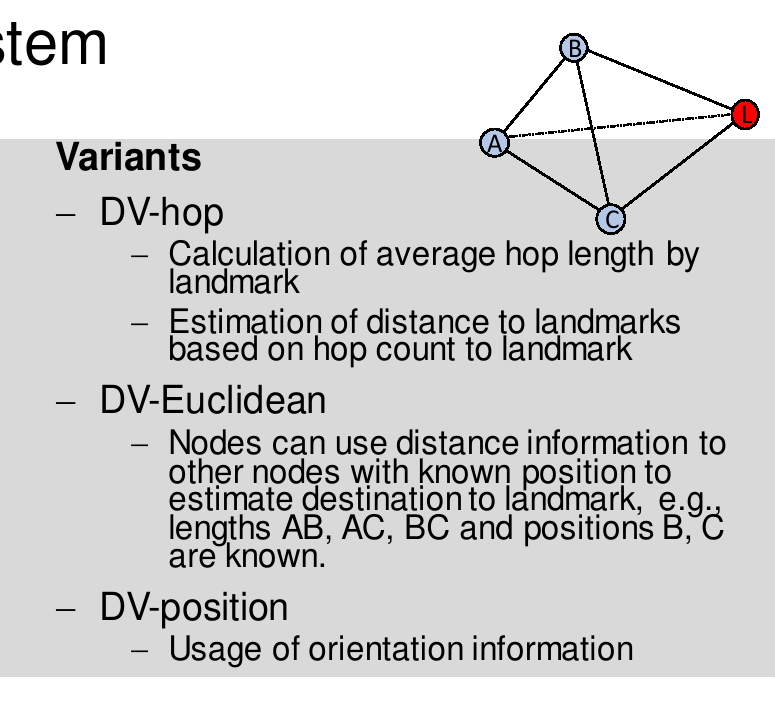
\includegraphics[width=0.6\textwidth]{04_adhoc_positioning}

\subsubsection{Ad-hoc localization}

\begin{itemize}
		\item Nodes learning their position via landmarks act as landmarks for other nodes
		\item Problem: If node not adjacent to more than 2 landmarks, not possible
		\item Approach: Have nodes collaborate to find groups where sufficient
				equations present to solve system
\end{itemize}


\section{Time synchronization}

Clocks must be synchronized to correlate events from different sensor nodes,
support synchronized sleep cycles, enable localization, ...

\begin{description}
		\item[Clock skew] Difference between reading of two clocks
		\item[Clock drift] Difference between reading of a clock and reference
				clock, per unit of time of reference clock
		\item[Send time] Time needed by packet from application to MAC layer,
				variable because of software delays.
		\item[Access time] Delay due to MAC protocol
		\item[Transmission time] Delay caused by bit transmission, follows from packet length and radio bandwith, deterministic
		\item[Propagation time] Signal propagation, follows from distance and speed of radio waves
		\item[Reception time] Time required to receive bits, deterministic
		\item[Receive time] Processing between MAC and application layer, variable
\end{description}

If drifts $d_{i, j}$ and initial offsets $o_{i, j}$ of two clocks are known,
then:
\begin{align*}
		c_i(t) & = d_i \cdot t + o_i \\
		c_j(t) & = d_j \cdot t + o_i
\end{align*}

Clock times can then be translated between two nodes:
\begin{align*}
		c_i(t) = a_{i, j} \cdot c_j(t) + b_{i, j}
\end{align*}

Where $a_{i, j}:= \frac{d_i}{d_j}$ and $b_{i, j} := - o_i \cdot a_i + o_{j, j}$.

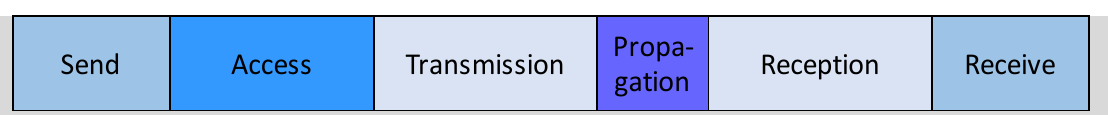
\includegraphics[width=\textwidth]{05_packet_delay}

\subsection{Classification of synchronization}

\begin{description}
		\item[Internal vs external synchronization] Synchronization among nodes vs with external master
		\item[Scope] All nodes vs subset
		\item[Rate vs offset synchronization] what is synchronized
		\item[Time-scale transformation vs clock synchronization] sync clocks or scale local time
		\item[Lifetime] Continuous vs on-demand
\end{description}

Synchronization schemes must be efficient (computational resources, energy,
..), precise, scalable, robust.

\subsection{GPS}

Requires line-of-sight. High power consumption of receiver. Requires four satellites.

\subsection{Time signals}

Time signals by dedicated radio stations. Low power consumption
(\SI{0.266}{\milli\watt} for \SI{1}{\hertz} receiver), error of
\SI{1}{\milli\second} with \SI{500}{\second} update interval on TelosB.

\subsection{Unidirectional synchronization}

Time-stamping of messages. Receiving node knows sending time of sender and
receiving time. Estimates delay $d$ as difference of the two.

\subsection{Roundtrip synchronization}

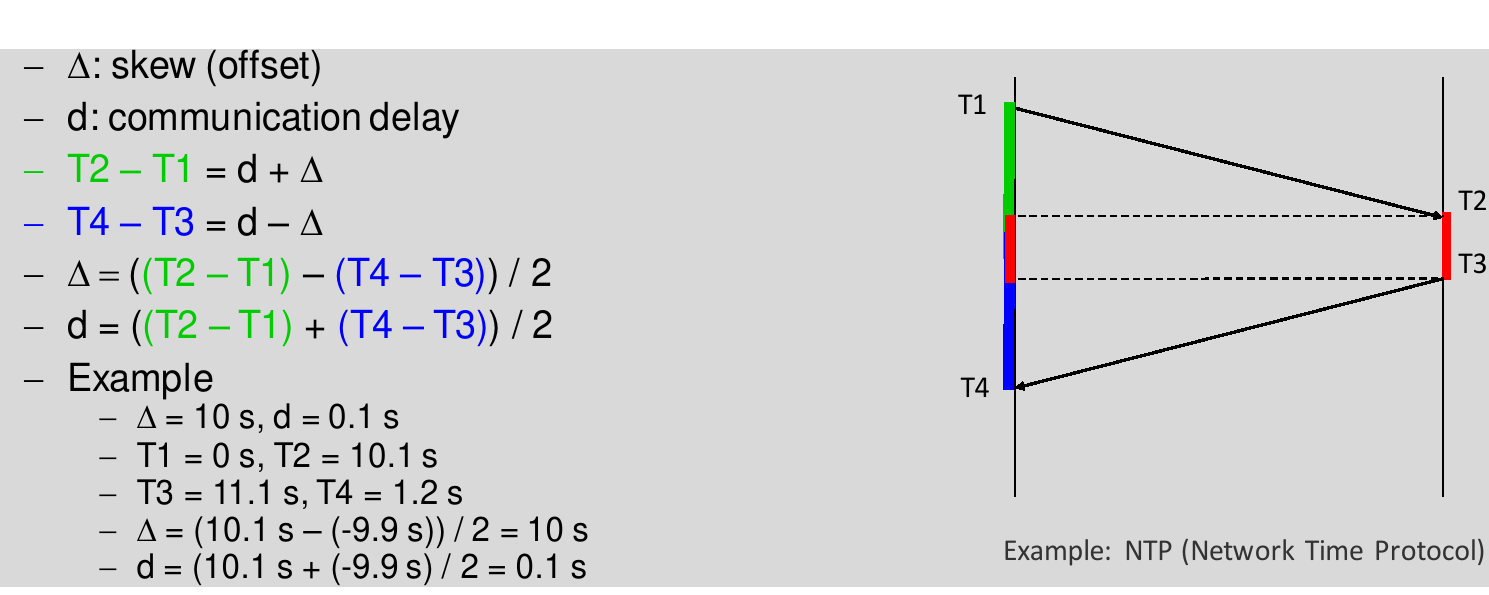
\includegraphics[width=\textwidth]{05_rt_sync}

\subsection{Reference broadcasting}

Can be used when master reaches two nodes, which cannot synchronize with each other.

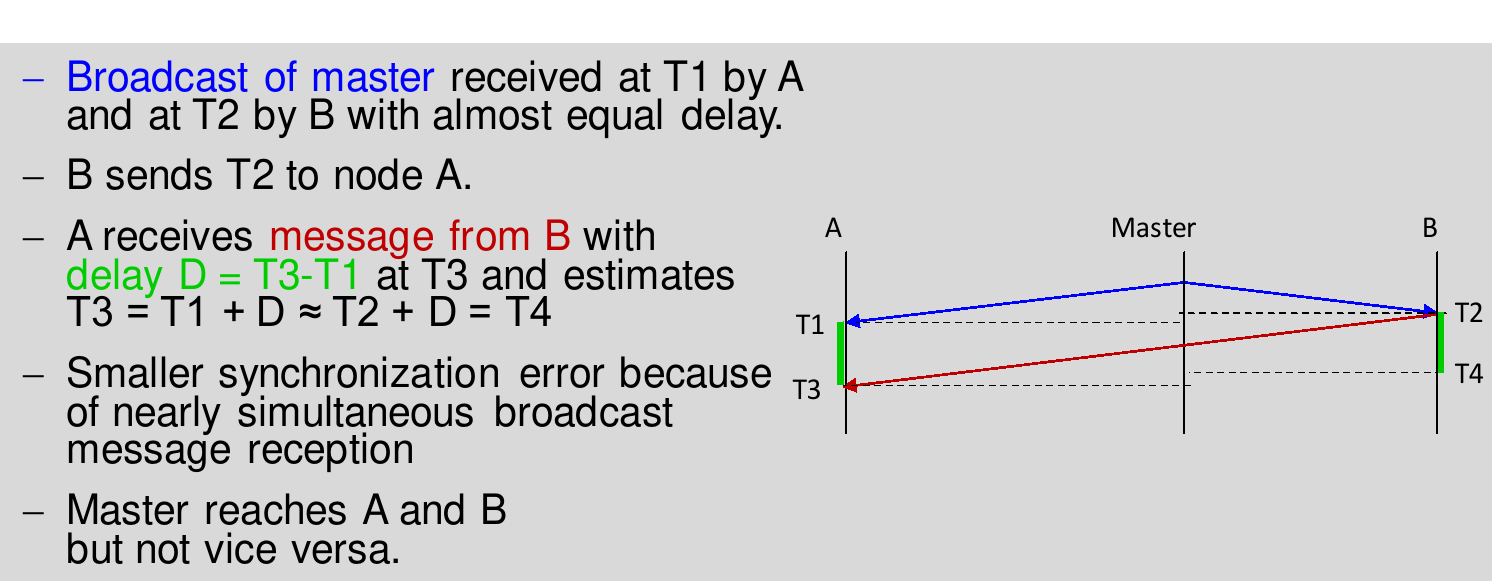
\includegraphics[width=\textwidth]{05_reference_broadcasting}

\subsection{Combining estimates}

Results of multiple synchronizations with same node can be combined using e.g.
linear regreission. Problem: Large memory requirements. Other approaches (e.g.
tiny-sync) more efficient although less accurate.

\subsection{Structured approaches}

Typically multiple nodes need to be synchronized which cannot communicate directly.

\subsubsection{Out-of-band synchronization}

Each node connected to at least one master which is synced to external system, eg GPS.

\subsubsection{Clustering}

All members of cluster can synchronize via e.g. reference broadcasting. Time
gateways (at least one per cluster) translate time stamps between clusters they
are part of. Tradeoff many translations vs large clusters (high power
consumption because of transmission range).

\paragraph{RBS}

Nodes send periodic beacons (pulses). Time difference between events and pulses
can be used to establish relationships.

\paragraph{Time routing in multi-hop networks with RBS}
Single time-gateways not desireable. Instead, dynamic time route establishment.
Each node converts time relationships before sending it on.

\subsubsection{Tree construction}

Synchronization tree with master as root. Single-hop synchronization along
tree. Accuracy degrades with distance from root.

\subsection{Unstructured approaches}

No structure established, completely localized solution.

\subsubsection{Diffusion-based synchronization}

Repeatedly perform steps which will eventually converge to shared time.k

\paragraph{Rate-based synchronous diffusion}

Random diffusion rates per pair of nodes, with sum $< 1$. Exchange time with
all neighbouring nodes. For each neighbour, adjust own time by delta with
neighbour, multiplied with rate: $c_i := c_i + r_{i, j} \cdot (c_j - c_i)$

\paragraph{Asynchronous diffusion}

Ask clock readings from set of random neighbours. Average readings (and use as
own?).  Send new value to neighbours.


\section{Topology coverage control}

Motivation: Roles need to be assigned to nodes. Nodes which aren't needed
should sleep.

\begin{description}
		\item[Topology coverage] Govern which nodes are required to provide
				communication network. Dependant on tx/rx capabilities.
		\item[Coverage control] Governs which nodes are required to cover
				desired area. Dependant on sensing capabilities.
\end{description}


\subsection{Topology coverage}

\begin{itemize}
		\item Must be energy-efficient, scalable, distributed, robust. Topology
				consists of set of active nodes $V$ and set of active links
				$E$.
		\item Topology control transform $(V, E)$ to $(V', E')$ by switching
				off (or back on) nodes in $V$, and limiting transmission power
				which will adjust $E$.
		\item Active links can be arranged hierarchical. Set of backbone nodes
				forming a ``connected dominating set'' (CDS). All non-backbone
				nodes connect only to backbone nodes. Backbone nodes may
				connect to anyone.
		\item Experiments show that, as transmission range increased, there's a
				certain point where connectivity (in percentage of total nodes
				reachable) rises sharply.  Ideally just above that point.
		\item Routing and topology control interact. E.g. if packet not
				deliverable, topology control must act.
\end{itemize}

\subsubsection{Flat topology control protocols}

\paragraph{Relative Neighborhood Graph, RNG}

RNG $T = (V, E')$ of graph $G = (V, E)$ is defined as:
\begin{align*}
		\forall u, v \in V: (u, v) \in E' \Leftrightarrow \not\exists w \in V: max(d(u, w), d(v, w)) < d(u, v)
\end{align*}

In words: Two nodes are connected IFF there is no other node that, if they were
connected via it, the longer of the two new connections would be shorter than
the existing one. Example: Edge between the blue ones not in RNG as each of the
blue-red edges would be shorter than the blue-blue one.

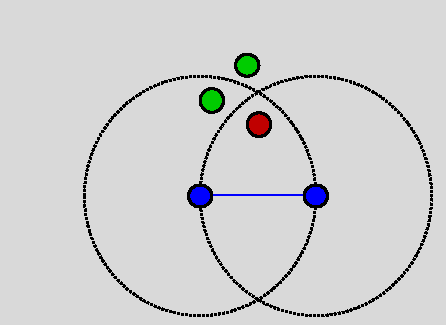
\includegraphics[width=0.5\textwidth]{06_rng}

\paragraph{Gabriel Graph, GG}

GG $T = (V, E')$ of $G = (V, E)$ is defined as:
\begin{align*}
		\forall u, v \in V: (u, v) \in E' \Leftrightarrow \not \exists w \in V : d^2(u, w) + d^2(v, w) < d^2(u, v)
\end{align*}

RNG is subgraph of GG.

\paragraph{Delaunay triangulation, DT}

The DT of a set of $n$ points $P$ is the unique triangulation such that the
cirumcircle of every triangle contains no points of $P$ in its interior.

\paragraph{Local Minimum Spanning Tree}

\begin{itemize}
		\item Beacons exchange information with max tx power, learn who their 1-hop neighbours are
		\item Construction of local minimum spanning tree \textbf{containing all 1-hop neighbours}
				\begin{itemize}
						\item Connections not necessarily the direct path! Can go via other neighbour.
				\end{itemize}
		\item Node $v$ is kept in neighbor list of node IFF it is a 1-hop
				neighbour \textbf{in its minimum spanning tree}
\end{itemize}

Example: Red is 1-hop neighbour of blue, but not 1-hop neighbour in its minimum
spanning tree, as cheaper connection via green (top right).

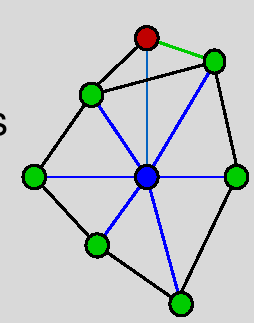
\includegraphics[width=0.5\textwidth]{06_lmst}

\paragraph{Cone-based topology control}

\begin{itemize}
		\item Each node splits its radial area into $n$ cones of angle $\alpha$
				(such that $n \cdot \alpha = 360$).
		\item Then, starting with a low TX power it sends beacons.
		\item Increases TX power until there's at least one neighbour in each cone.
		\item If there are two edges $(u, v_1)$, $(u, v_2)$, the longer can be
				removed if $d(v_1, v_2) < max(d(u, v_1), d(u, v_2))$
\end{itemize}


\paragraph{COMPOW}

\begin{itemize}
		\item Assume node has power levels
		\item Node selects lowest power level having same number of reachable
				nodes as maximum power level
		\item Enabled by one routing protocol per power level. But causes
				overheads, as multiple routing layers active.
\end{itemize}

\subsubsection{Hierarchical topology control}

Idea: Select virtual backbone of nodes which remain active.

\paragraph{Minimum connected dominating sets, MCDS}

Dominating set is subset $D$ of $V$ where each node in $V \setminus D$ is
adjacent to some node in $D$. That is every node eitehr is in D, or has an edge
connecting it to a node in D.

Connected dominating set is a dominating set which builds a connected sub-graph
of the network.

Minimum cds is the CDS containing the least amount of nodes. Finding it is
NP-complete, but heuristics exists, such as MPR-CDS.

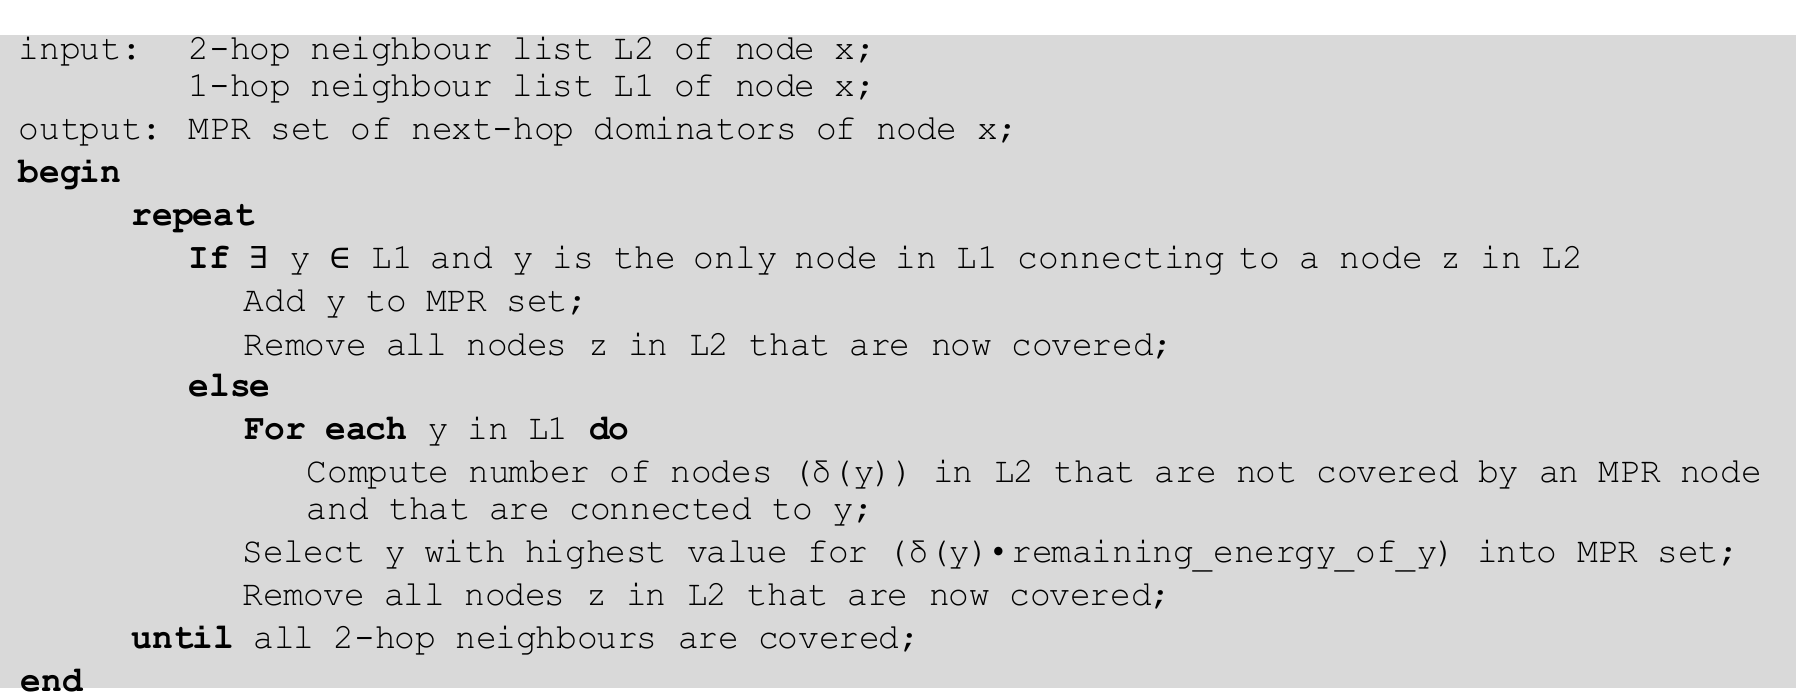
\includegraphics[width=\textwidth]{06_mpr_cds}

\paragraph{SPAN}

\begin{itemize}
		\item Node periodically announces willingness to become coordinator
				(part of backbone) if it discovers that two neighbours cannot
				communicate via at most 2 backbone nodes.
		\item When node wants to withdraw as coordinator it announces itself as
				tentative. If none objects, it withdraws.
		\item Randomized back-off delay for announcements.
\end{itemize}

\paragraph{Geographic adapative fidelity}

\begin{itemize}
		\item Nodes on virtual grid, can communicate if in adjacent cells
		\item One node per cell chosen to always be active
		\item Active node sleeps if more suitable node detected, based on e.g.
				node lifetime.
\end{itemize}

\subsection{Coverage control}

\subsubsection{Probeing Environment and Adaptive Sleeping, PEAS}

\begin{itemize}
		\item Sensor nodes sleep, wake up periodically, send probing message
		\item Receiving sensors estimate distance to probing sensor. If too
				close they announce their presence, probing node sleeps again.
		\item Otherwise, probing node becomes active
		\item Probing frequency balances energy usage and robustness
\end{itemize}

\subsubsection{Node-self-scheduling scheme, NSSS}

\begin{itemize}
		\item Node measures neighbourhood redundancy as union of sectors covered by neighbouring sensors
		\item If full \SI{360}{\degree} covered, node can withdraw
		\item Problem: Node failures
\end{itemize}

\subsubsection{Gur Game}

\begin{itemize}
		\item Sensors run FSM split in two halves. Left: No data sent. Right: Data sent.
		\item Base station calculates and broadcasts $r = f(\text{received
				packets})$, which is function which max at desired number of
				packets.
		\item Nodes move, with probability $r$, towards the edge, with $1 - r$
				towards the center of the FSM.
\end{itemize}

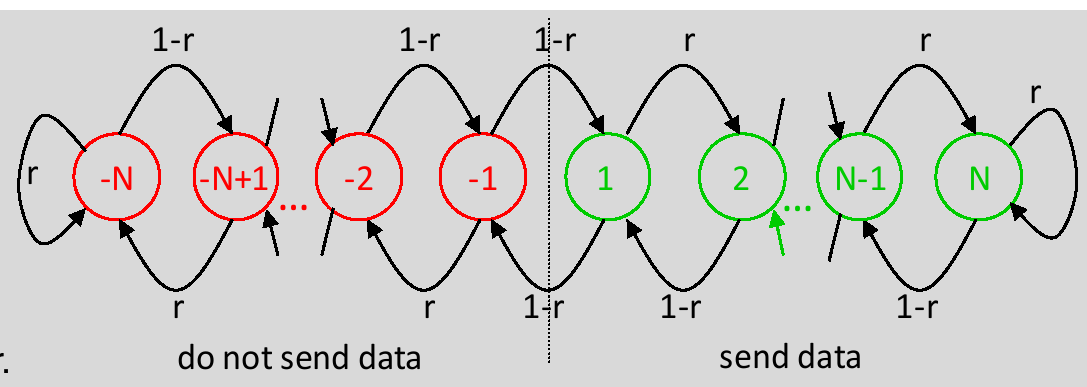
\includegraphics[width=\textwidth]{06_gur_game}

\subsubsection{Reference time-based scheduling scheme}

\begin{itemize}
		\item Divide environment into grid. Assume tx radius > 2 sensing radius
		\item Broadcast randomly chosen reference time in $[0, T)$, $T$ round length
		\item For each grid point, sensor sorts reference time of sensors able to monitor (= reach) it
		\item Schedules its own activity centered on its own reference time,
				such that it reaches at most halfway towards the next lower and
				higher reference times.
\end{itemize}

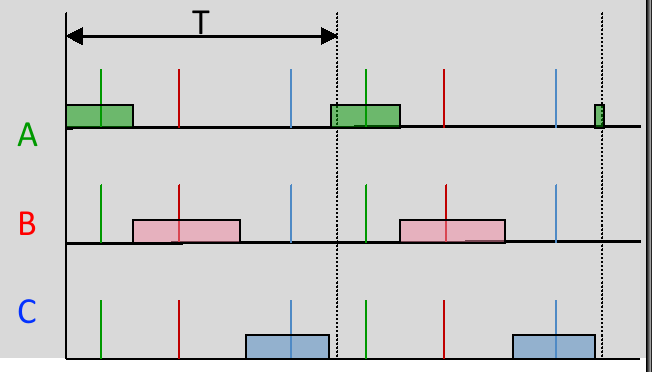
\includegraphics[width=\textwidth]{06_reference_time}

\subsubsection{Coverage configuration protocol, CCP}

\begin{itemize}
		\item Node determines intersection points between coverage area and neighbours' sensing radii
		\item Node sleeps if each intersection point covered by at least $k$ neighbours
\end{itemize}

\subsection{Combining topology and coverage control}

Problem: Topology control has no knowledge of traffic patterns. Often traffic
from select few nodes, and topology control maintains too big a communication
network.

\subsubsection{Connected sensor cover}

Idea: Find minimum number of nodes to cover area.

\begin{itemize}
		\item If $M$ set of covered sensors
		\item Find candidates with sensing region intersecting that of M
		\item Find path $P_i$ to every candidate (starting in M) with highest
				benefit (additional coverage for $M$)
		\item Add path with highest benefit, add candidates along that path
\end{itemize}

\subsubsection{Distributed activation with pre-determined routes}

Idea: Important or low-energy nodes should not be used for sensing.

\begin{itemize}
		\item Each node assigns itself a cost
		\item Route discovery using cost as routing metric
		\item Nodes activate themselves after back-off delay proportional to activation cost. No activation if neighbourhood covered
		\item Nodes deactivate themselves if they discover redundant nodes.
\end{itemize}


\section{MAC}

Goal: Resource-efficient collision avoidance. Scalable, robust and fair.
Collisions and overhearing cause lots of energy loss, so should be avoided.

\begin{description}
		\item[Scheduled protocols]: Polling (central controller allocates
				slots) vs multiplexing (pre-allocated channels), but causes
				overhead (polling) or not scalable (multiplexing)
		\item[Contention-based protocols] On-demand sharing of channels, but
				inefficient in times of contention
		\item[Hybrid approaches] Combining scheduled and contention-based
\end{description}

\subsection{Scheduled protocols}

Access scheduled. Collision-free, but costly to maintain, requires synchronized
nodes.

\subsubsection{Based on clustesr}

Idea: Form clusters, one node acts as cluster head and schedules access. Nodes
only communicate with cluster head.

\paragraph{Low Energy Adaptive Clustering Hierarchy, LEACH}

\begin{itemize}
		\item Nodes organize into clusters with rotating heads. Only active
				when transmitting.
		\item Cluster heads always active. Calculate schedule for nodes,
				aggregate data and forward to sink.
		\item Cluster head election once per round. Each nodes elects self with
				certain probability, dependant on e.g. energy level. Other
				nodes then join cluster head with strongest signal.
\end{itemize}

\subsubsection{Self-organizing}

\begin{itemize}
		\item Nodes find each other on fixed frequency, agree on pair of slots
				to transmit and receive. Leads to a frequency/time/mode tuple
				for each pair of nodes.
\end{itemize}

\subsubsection{Lightweight MAC}

\begin{itemize}
		\item Time-based multiplexing, based on choices of 1-hop neighbours
\end{itemize}

\subsection{Contention-based protocols}

Shared channels. ALlocation on demand. Flexible and scalable, no need for
synchronicity, but potentially inefficient when there is contention.

\subsubsection{Wakeup radio}

\begin{itemize}
		\item Idle channel randomly chosen. If no idle channel available, random backoff.
		\item Low-power control channel indicates upcoming transmission, wakes
				nodes from sleep if they are destination.
\end{itemize}

\subsubsection{Periodic wakeup}

\begin{itemize}
		\item Receiving node periodically wakes up. Requires sending node to know about duty cycles.
		\item Or sending node must announce transmission ahead of time
		\item Or send long preamble (> sleep cycle)
		\item Or receiving node announces its wake time
		\item Or time synchronization
\end{itemize}

\begin{description}
		\item[X-MAC] Preamble including address, receiver acks preamble, then data follows
		\item[BEAM] Long or short preambles with/without payload. Receiver acks
				preamble (if without payload) or full data frame (if with
				payload). Preamble in the front allows non-intended receivers
				to sleep early.
		\item[B-MAC] Long preamble followed by data. Receiver periodically
				wakes to listen for preamble.
		\item[WiseMAC] Sender sends preamble prior to data packet, nodes
				periodically check medium. If medium busy, they receive. Nodes
				tell each other about sampling schedule via ACKs.
		\item[ContikiMAC] Combination of B-MAC (low-power listening), X-MAC
				(preamble), BEAM (data packets), WiseMAC (receiver wakeup time
				estimation)
		\item[Maximally Traffic-Adaptive and energy-efficient MAC] Sampling of
				preambles like WiseMAC, change sampling frequency by frequency
				of recently received packets.
		\item[Receiver-initiated MAC] Source becomes active, listens to
				destination's beacon. Once received it sends data. Destination
				acks.
		\item[Sensor MAC] Each node picks and periodically broadcasts its
				sleep/listen schedule. If it receives another's schedule it
				adopts it. If no other neighbours it adopts it exclusively, if
				other neighbours then it attempts following both.
		\item[Traffic-aware energy-efficient MAC] Optimizes S-MAC by combining
				SYNC and RTS.
\end{description}

Max-MAC:
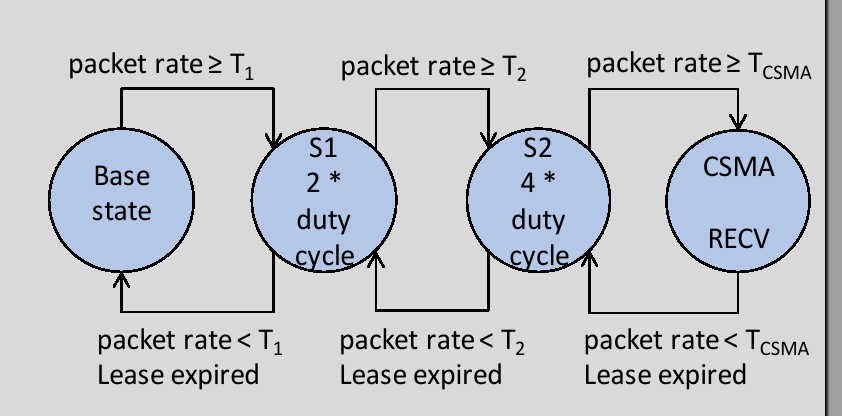
\includegraphics[width=0.5\textwidth]{07_max_mac}

Sensor MAC
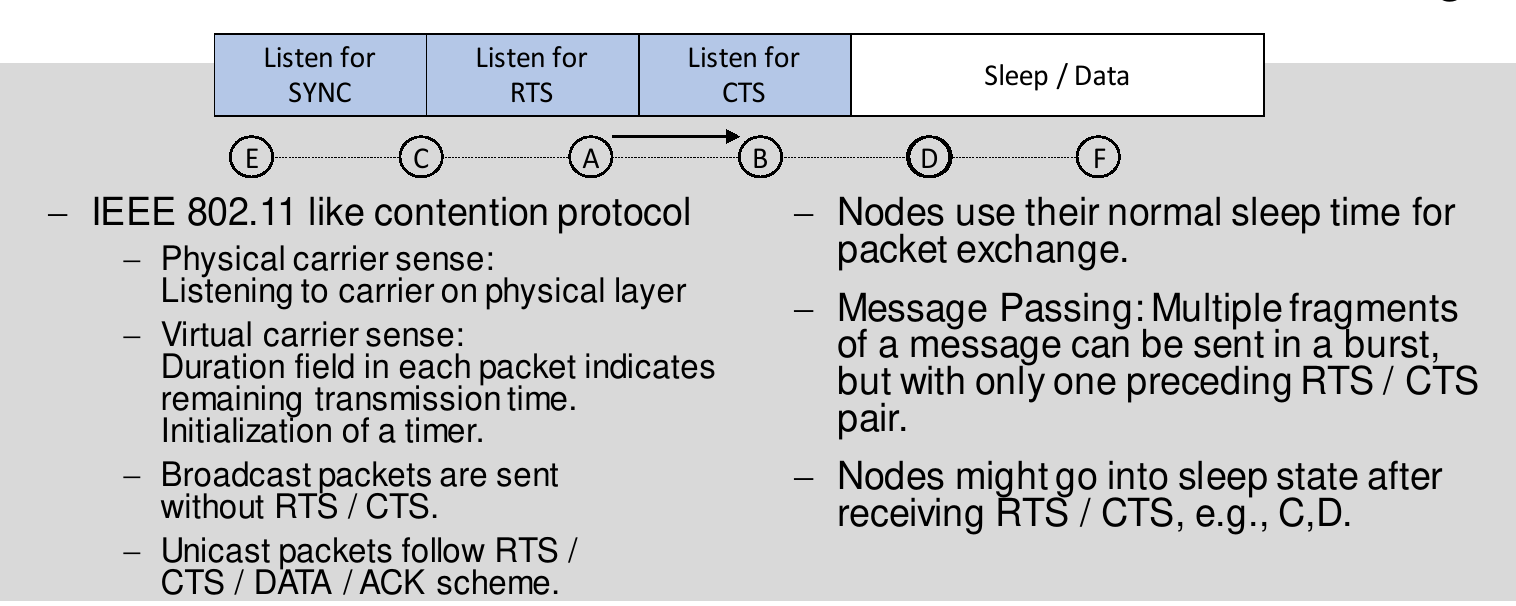
\includegraphics[width=\textwidth]{07_smac}

\subsection{Industry standards}

\subsubsection{IEEE 802.15.43, Low-rate wireless PAN}

Specifies wireless MAC and physical layer for low-rate WPAN. Contiki only uses
physical layer, not MAC layer. Standard is basis for e.g. ZigBee and WirelessHART.

\begin{itemize}
		\item OTA data rates of up to \SI{250}{kbps}
		\item Optional allocation of guaranteed time slots
		\item Carrier-sense multiple access with collision avoidance
		\item Link quality indication
		\item Two types of device: Full-function which can operate as
				coordinator. Reduced-function, which only works as device.
		\item FFD can talk to RFD and FFD, RFD only to FFD.
		\item Forms tree-like structures with RFDs in leaves, FFDs in other
				places.
\end{itemize}

\paragraph{Slot structure}

Coordinator defines slots. Some for contention-based access (with e.g.
listening), some with guaranteed (scheduled) access. Part of the superframe can
also be empty, allowing coordinator to sleep.

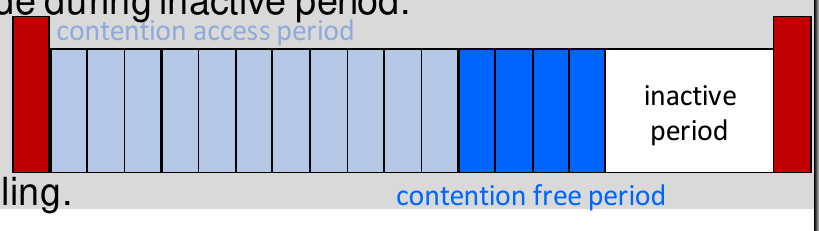
\includegraphics[width=0.5\textwidth]{07_ieee}

\paragraph{Low-energy mechanisms}

\begin{description}
		\item[Coordinated sampled listening] Receiving and transmitting devices
				coordinate sampling times to reduce overhead.
		\item[Receiver-initiated transmission] Receiving devices beacon data
				request, transmitting devices only transmit when such a beacon
				received.
\end{description}

\subsubsection{Wireless HART}

\begin{itemize}
		\item Fore wireless sensor networks, based on IEEE 802.15.4 physical layer
		\item TDMA MAC with rigid time synchronization requirement across entire network
		\item \SI{10}{ms} slots
\end{itemize}

\subsubsection{LoraWAN}

\begin{itemize}
		\item Secure bidirectional communication
		\item Star-of-stars topology
		\item End devices use single-hop communication to one or many gateways
		\item LoraWAN network server manages data rate and RF output of each end-device
\end{itemize}

Three types of devices:

\paragraph{Class A, battery powered}

\begin{itemize}
		\item Picks its own transmission slot, with small random variation
		\item Opens two receive windows
\end{itemize}

\paragraph{Class B, low latency}

\begin{itemize}
		\item Scheduled receive slots assigned by beacon from gateway
		\item Unicast and multicast
\end{itemize}

\paragraph{Class C, no latency}

\begin{itemize}
		\item Nearly continuous receive window, only closed when transmitting
		\item Unicast and multicast
\end{itemize}

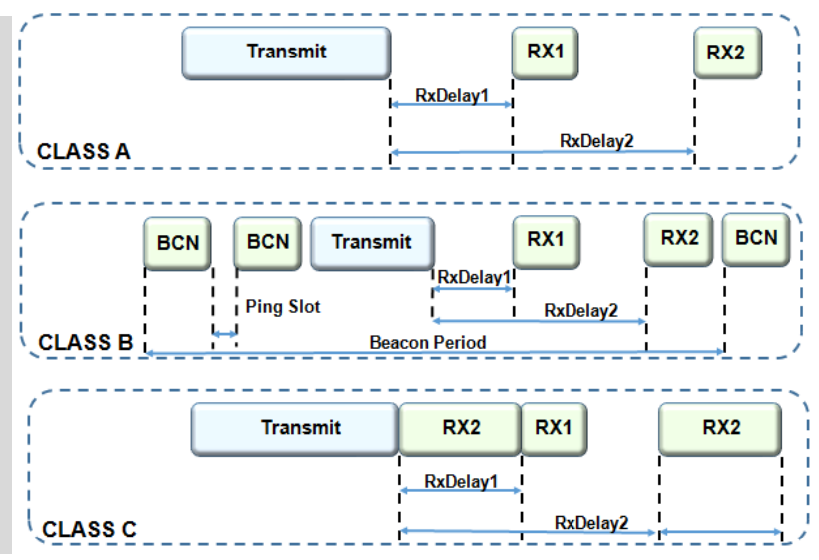
\includegraphics[width=0.6\textwidth]{07_lorawan}


\clearpage

\end{document}

